\documentclass[11pt]{article}
\usepackage[margin=1in]{geometry}
\usepackage{graphicx}
\usepackage{amsmath}
\usepackage{booktabs}
\title{A Finite Intercept Correction Calculation}
\author{Anonymous}
\date{}
\begin{document}
\maketitle
\begin{abstract}
This synthetic teaching note documents a reproducible intercept correction on five observations. Inputs $x=(-2,-1,0,1,2)$ have targets $y=2x+3$, whereas a fixed predictor returns $2x$. Averaging the observed residuals gives an additive correction $b=3$, reducing recorded mean squared error from $9$ to $0$. An intermediate correction, an error table, and two figures expose the calculation. The same observations determine and evaluate the correction; these results demonstrate finite arithmetic without establishing predictive generalization or algorithmic novelty.
\end{abstract}
\section{Introduction}
A constant prediction error can be illustrated through a finite calculation in which the prediction rule omits an additive term. This teaching note considers five inputs,
\[
x_i \in \{-2,-1,0,1,2\},
\qquad y_i=2x_i+3,
\]
and the fixed predictor $\hat{y}_i=2x_i$. On each of these observations, the target minus the prediction is exactly $3$. The example therefore isolates the effect of an omitted intercept while keeping the coefficient of $x$ fixed.

The correction is obtained directly from the observed residuals:
\[
b=\frac{1}{5}\sum_{i=1}^{5}(y_i-2x_i)=3,
\qquad
\hat{y}_i^{\mathrm{corr}}=2x_i+b.
\]
The recorded calculation compares the three additive values $b=0$, $b=1.5$, and $b=3$. Their mean squared errors are $9$, $2.25$, and $0$, respectively; their mean absolute errors are $3$, $1.5$, and $0$. These values describe the arithmetic on the five listed observations.

The purpose of the note is to make the residual-to-correction computation transparent, not to introduce a new algorithm or establish a research advance. The calculation is implemented in base R and involves no optimizer or stochastic repetitions. Crucially, the same five observations determine the correction and measure its error. The zero recorded error at $b=3$ demonstrates exact agreement on these observations, but supplies no measurement of predictive performance on other observations.

\section{Related Work}
This note makes no literature-based claim of novelty and reports no comparison with external methods. The discussion below identifies the conceptual scope of the calculation and the limits of its evaluation.

\subsection{Fixed Predictors and Additive Offset Corrections}
The example concerns a fixed prediction rule supplemented by a single scalar offset. The coefficient multiplying $x$ remains $2$ throughout; only the added value changes. For the five observations considered here, every residual $y_i-2x_i$ equals $3$, so averaging the residuals returns that same value. Adding it to the predictions removes the observed discrepancy at every listed point.

This correspondence depends on the constant residual in the specified example. The calculation does not examine observations with varying residuals, estimate a different slope, or compare alternative correction procedures. Its role is to illustrate how the observed constant discrepancy becomes an additive correction. The three recorded settings, $b=0$, $b=1.5$, and $b=3$, are the complete measured comparison.

\subsection{Evaluation of Corrections Estimated from Observed Residuals}
The correction depends on the observed targets through the residuals used to compute its mean. Evaluating $2x_i+b$ on those same observations therefore measures agreement with the data that supplied $b$. In this example, exact agreement follows from the shared residual value of $3$.

The experimental record contains no evaluation on separate observations. Consequently, the reported errors support only the finite comparison among the three recorded offsets. They do not establish generalization, robustness to other residual patterns, or superiority over an external method. Making the dependency between correction estimation and evaluation explicit is part of the teaching purpose of this note.
\section{Method}
\subsection{Finite Observations and Residual Correction}
Index the supplied inputs in order by $i=1,\ldots,5$. Their targets and baseline predictions are
\[
(y_i)_{i=1}^{5}=(-1,1,3,5,7),
\qquad
(2x_i)_{i=1}^{5}=(-4,-2,0,2,4).
\]
Thus $r_i=y_i-2x_i=3$ for every index. The correction is
\[
b=\frac{1}{5}\sum_{i=1}^{5}r_i=3,
\]
giving $\hat{y}_i^{\mathrm{corr}}=2x_i+3=y_i$. This is direct arithmetic with a fixed slope.

\subsection{Error Calculation and Data Dependency}
For an added value $b$, define the evaluation residual as
$e_i(b)=y_i-(2x_i+b)=3-b$. On these observations,
\[
\begin{aligned}
\operatorname{MAE}(b)
&=\frac{1}{5}\sum_{i=1}^{5}|e_i(b)|=|3-b|,\\
\operatorname{MSE}(b)
&=\frac{1}{5}\sum_{i=1}^{5}e_i(b)^2=(3-b)^2.
\end{aligned}
\]
These identities explain the three recorded settings. Figure~\ref{fig:residual_workflow} traces the dependency from observed residuals to $b$ and the reuse of targets for evaluation. Base R implements the calculation; the supplied schematic uses LaTeX/TikZ.

\begin{figure}[htbp]
    \centering
    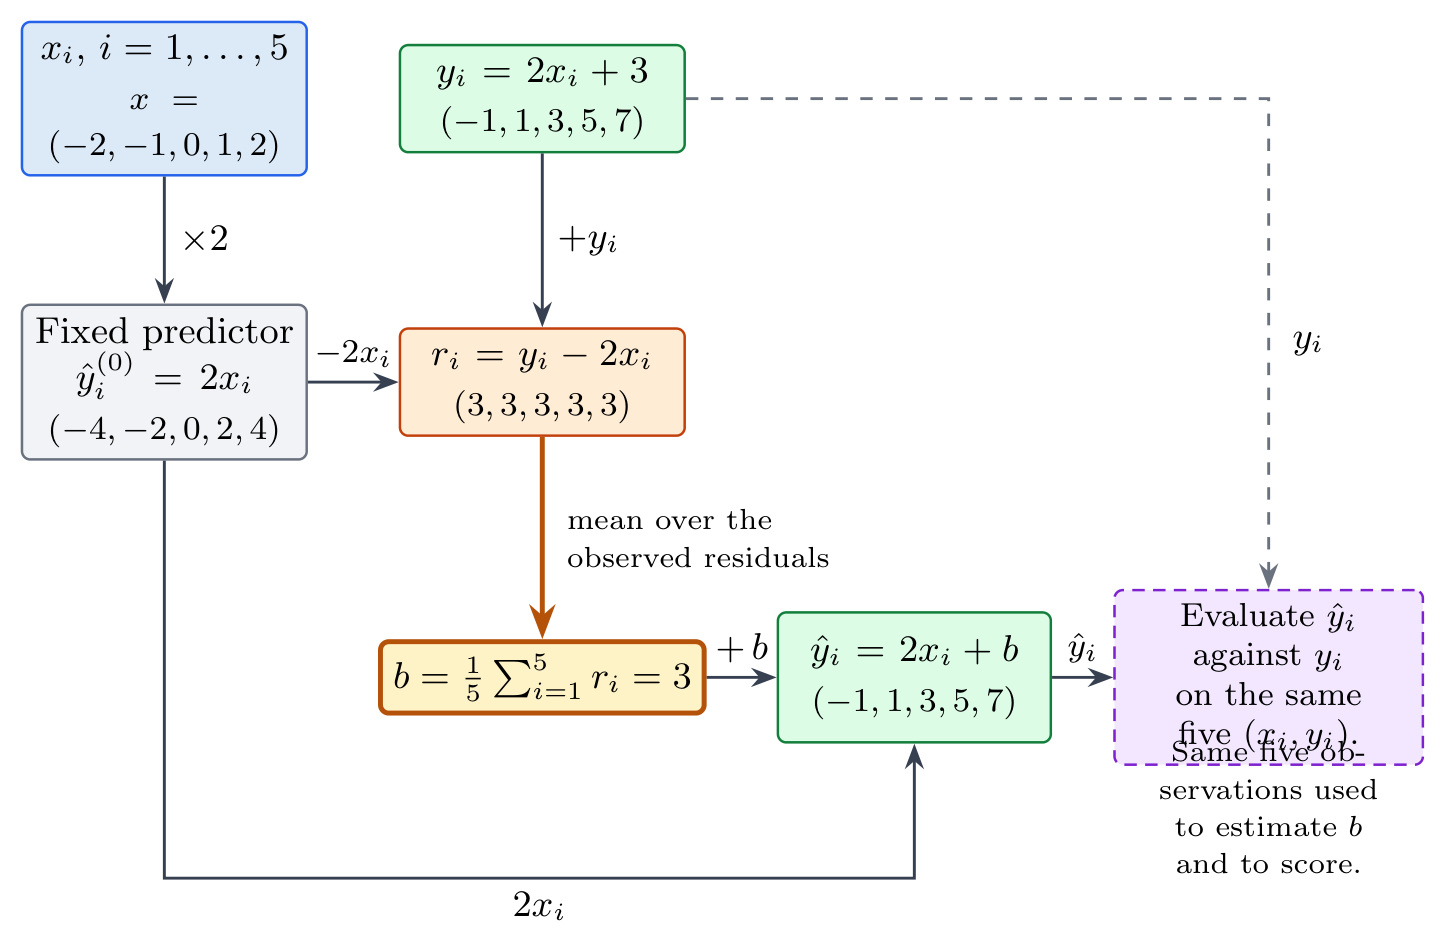
\includegraphics[width=\linewidth]{figures/fig_residual_workflow.jpg}
    \caption{Observed residuals determine the scalar correction $b=3$, which is added to the fixed predictions. The same five observations supply the evaluation targets.}
    \label{fig:residual_workflow}
\end{figure}

\section{Experiments}
\subsection{Deterministic Calculation and Recorded Results}
The experimental record contains one deterministic calculation on five supplied synthetic observations. Table~\ref{tab:errors} reproduces its complete error comparison.

\begin{table}[htbp]
    \centering
    \caption{Recorded errors on the five observations used to determine the correction.}
    \label{tab:errors}
    \begin{tabular}{rrr}
        \toprule
        Added $b$ & Mean absolute error & Mean squared error \\
        \midrule
        0   & 3   & 9    \\
        1.5 & 1.5 & 2.25 \\
        3   & 0   & 0    \\
        \bottomrule
    \end{tabular}
\end{table}

The offset comparison isolates the effect of changing $b$: the uncorrected predictor retains residual $3$, while $b=1.5$ leaves residual $1.5$ at every point. This intermediate setting halves MAE and quarters MSE relative to $b=0$; it is a recorded partial correction, not a separately learned method or stochastic ablation. At $b=3$, the corrected predictions $(-1,1,3,5,7)$ match all five targets in the observation-level log. Exact cancellation follows because the discrepancy is constant.

\subsection{Visualization, Reproducibility, and Interpretation}
Figure~\ref{fig:intercept_error} displays exactly the three recorded MSE values using R/ggplot2. Its isolated points add no measurements between settings. No uncertainty estimates, significance tests, convergence measurements, timing results, or held-out results are recorded. The evidence therefore verifies arithmetic on the supplied observations.

\begin{figure}[htbp]
    \centering
    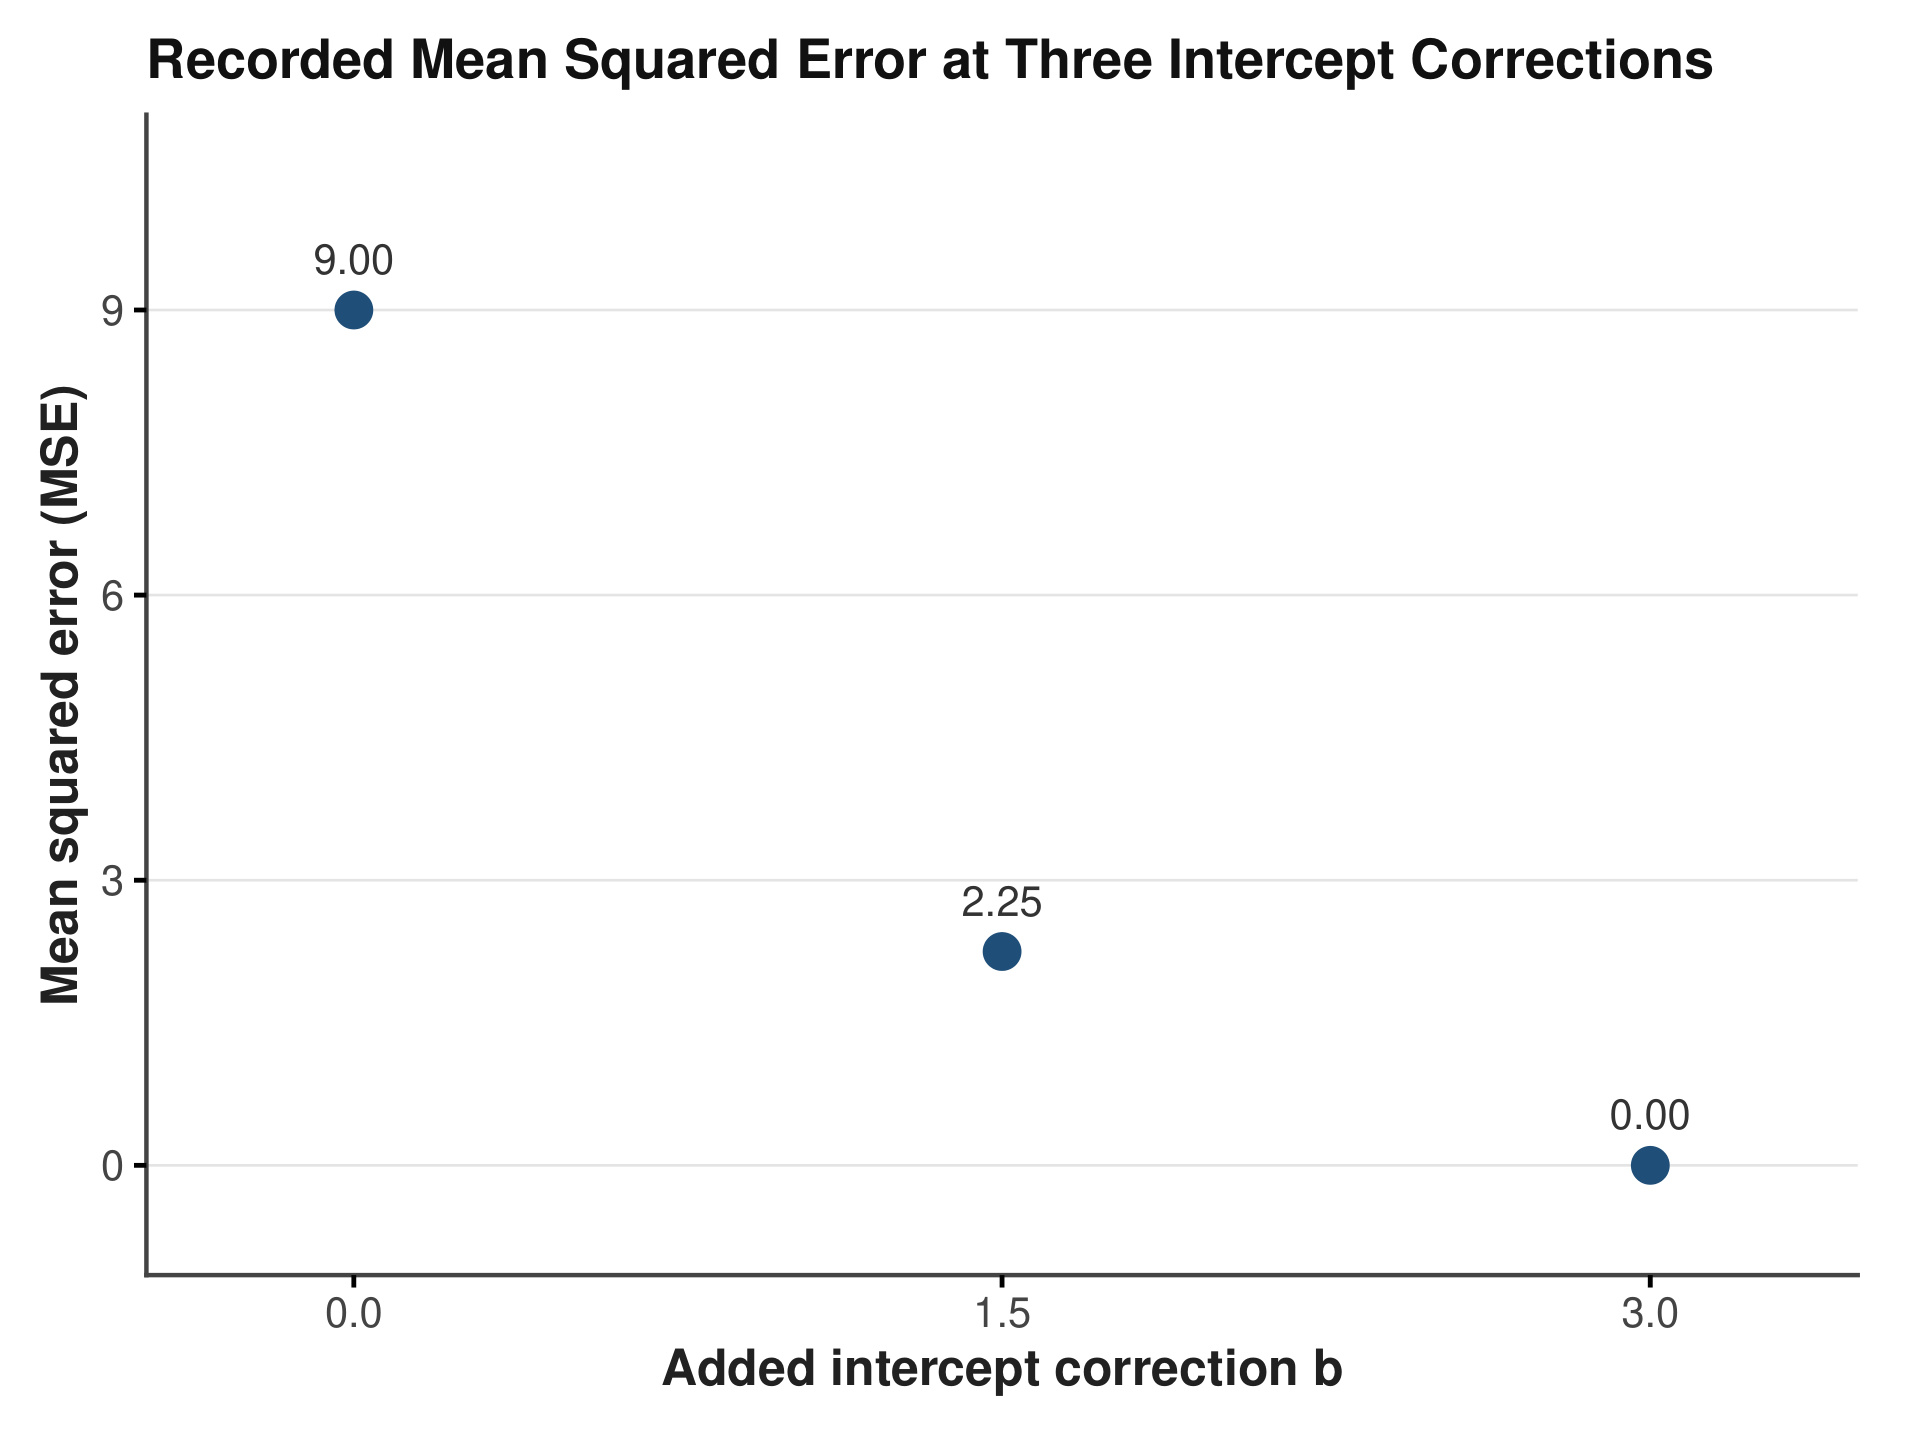
\includegraphics[width=\linewidth]{figures/fig_intercept_error.jpg}
    \caption{Recorded MSE at $b=0$, $1.5$, and $3$. The same five observations determine and evaluate the correction, so the points demonstrate finite arithmetic rather than predictive generalization.}
    \label{fig:intercept_error}
\end{figure}

\subsection*{Figure source provenance}
The selected figures retain their supplied editable sources:
\begin{itemize}
    \item \texttt{\detokenize{figure_code/fig_intercept_error/source.R}}
    \item \texttt{\detokenize{figure_code/fig_residual_workflow/source.tex}}
\end{itemize}
Their respective directories retain vector \texttt{figure.pdf} files, manuscript-compatible \texttt{preview.jpg} files, and renderer inputs. These source artifacts accompany the supplied images without reconstructing or replacing their figure recipes.

\clearpage
\section{Conclusion}
Adding the observed mean residual $b=3$ changes recorded MAE and MSE from $3$ and $9$ to $0$ and $0$ on the same five points. The table and figures make this teaching calculation inspectable and reproducible. No separate observations were evaluated, so the result establishes only exact agreement on the supplied observations. Future evaluation on separate observations would be needed to assess performance beyond this finite calculation.

\bibliographystyle{plain}
\bibliography{references}

% PAPER_ORCHESTRA_PROVENANCE_BEGIN
\clearpage
\section*{Figure source provenance}
The files below are the exact sources that produced the embedded figure previews. Paths are relative to this manuscript's source directory. The accompanying \texttt{figure\char95{}provenance.json} records all artifact checksums.\par
\medskip\noindent\textbf{Figure~\ref{fig:intercept_error} (\texttt{fig\char95{}intercept\char95{}error.jpg}).}\par
\noindent R/ggplot2 source: \texttt{figure\char95{}code/\allowbreak{}fig\char95{}intercept\char95{}error/\allowbreak{}source.R}.\par
\noindent Source SHA256: \texttt{18933984\allowbreak{}6a19ff9a\allowbreak{}fe13e24a\allowbreak{}7efe95cc\allowbreak{}4a83ec38\allowbreak{}a9778113\allowbreak{}caa8f8c9\allowbreak{}2dd0589a}.\par
\noindent Rendering metadata: \texttt{figure\char95{}code/\allowbreak{}fig\char95{}intercept\char95{}error/\allowbreak{}render.json}.\par
\noindent Exact export wrapper: \texttt{figure\char95{}code/\allowbreak{}fig\char95{}intercept\char95{}error/\allowbreak{}worker.R}.\par
\noindent Wrapper SHA256: \texttt{6cb2b073\allowbreak{}27277f63\allowbreak{}fafbb553\allowbreak{}cd4f1f12\allowbreak{}c0f85bec\allowbreak{}37a49f3f\allowbreak{}a765da16\allowbreak{}a26b58ba}.\par
\noindent Rendering metadata: \texttt{figure\char95{}code/\allowbreak{}fig\char95{}intercept\char95{}error/\allowbreak{}sessionInfo.txt}.\par
\medskip\noindent\textbf{Figure~\ref{fig:residual_workflow} (\texttt{fig\char95{}residual\char95{}workflow.jpg}).}\par
\noindent LaTeX/TikZ source: \texttt{figure\char95{}code/\allowbreak{}fig\char95{}residual\char95{}workflow/\allowbreak{}source.tex}.\par
\noindent Source SHA256: \texttt{4e19b72b\allowbreak{}be6333b3\allowbreak{}602153f3\allowbreak{}eab1b16a\allowbreak{}e392856f\allowbreak{}fa6a5527\allowbreak{}ea378e37\allowbreak{}911eb5fe}.\par
\noindent Rendering metadata: \texttt{figure\char95{}code/\allowbreak{}fig\char95{}residual\char95{}workflow/\allowbreak{}render.json}.\par
% PAPER_ORCHESTRA_PROVENANCE_END
\end{document}